\documentclass{article}

%\usepackage{mathtools}
\usepackage{amsfonts}
\usepackage[spanish,mexico]{babel}
\usepackage[utf8]{inputenc}
\usepackage{graphicx}
\usepackage{url}
\usepackage{listings}%http://www.tex.ac.uk/FAQ-codelist.html
\lstset{language=Python}
\graphicspath{ {programas/img/} }
%\usepackage{enumitem}
%\usepackage{tikz}

\title{Representación mediante grafos de un problema de asignación de horarios}
\author{José Alberto Benavides Vázquez}
\date{\today}

\begin{document}

  \maketitle

  Supongamos una institución educativa que ofrece materias presenciales a sus alumnos y que debe asignarles horarios a esas materias para que los alumnos interesados en ellas puedan asistir a clases. Si dicha institución tiene una cantidad determinada de horarios para asignar a las materias ofertadas y un límite de salones disponibles donde ubicar físicamente a los grupos de esas materias, podría darse el caso de que un mismo alumno esté interesado en materias distintas que compartan el mismo horario pero en distintos salones. Si además la institución desea que sus alumnos puedan inscribir cuantas materias les interesen, esto supondría un problema para la institución y los alumnos. Este problema podría resolverse mediante grafos.

  Un grafo es una representación de elementos cualesquiera y de los posibles vínculos que pudiera haber entre ellos mediante puntos y líneas, llamados nodos y arcos respectivamente. Estos nodos y arcos podrían representarse de maneras diferentes para distinguir entre los elementos y los vínculos que simbolizan. Por ejemplo, una calle recta que comunica dos casas podría representarse con un nodo en la izquierda de un color, un nodo en la derecha de otro color y una línea recta que los conecte como en la figura \ref{fig:carrera}.

  \begin{figure}[h] % https://es.sharelatex.com/learn/Inserting_Images
    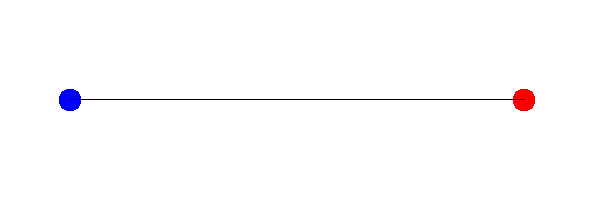
\includegraphics[width=0.7\textwidth]{carrera}
    \centering
    \caption{Representación de una calle (línea negra) que conecta dos casas (una azul a la izquierda y una roja a la derecha).}
    \label{fig:carrera}
  \end{figure}

  De esta manera, muchas situaciones podrían representarse simplemente mediante grafos ~\cite{BarabasiNetwork}. En esta ocasión, para representar el problema de asignación de horarios mencionado al inicio se ha optado por hacer un código en Python que generara una salida para ser recibida por Gnuplot que diera por resultado una imagen PNG, lo cual forma parte de los objetivos del curso Optimización de flujo en redes ~\cite{SchaefferNetwork} para el que se realiza este reporte.

  Se desarrolló un programa que toma como valores iniciales:

  \begin{itemize}
    \item $A$: cantidad de alumnos inscritos,
    \item $M$: número de materias registradas,
    \item $H$: total de horarios disponibles y
    \item $p_h$: probabilidad de que un horario sea asignado a cualquier materia.
  \end{itemize}

  Posteriormente, se generaron aleatoriamente probabilidades $p_m, \forall m \in M$ de que cada materia fuera interesante para cualquier alumno y se comparó para cada alumno y materia con una probabilidad $p_{am}$ generada al azar de que a cada alumno le interesara cierta materia, de modo que si $p_{am} < p_m, \forall a \in A, \forall m \in M$, se creara una pareja de interés alumno-materia, comparación que se repitió hasta que todos los alumnos estuvieran al menos interesados en una materia.

  A continuación, se establecieron parejas materia-horario comparando la probabilidad $p_h$ de que a un horario se le asignara cualquier materia,  con una probabilidad $p_mh$ generada al azar de que a una materia se asignara cierto horario, tal que si $p_{mh} < p_h$ se asignaría a la materia $m$ el horario $h$, lo cual se repetiría para cada materia hasta que todas las materias tuvieran un solo horario asignado.

  Una vez generadas estas parejas alumnos-materias y materias-horarios, se optó por la representación mediante nodos de los alumnos, materias y horarios, mientras que las relaciones entre estos nodos se mostrarían por arcos. Así, cada alumno interesado en una clase y cada materia inscrita en un horario formarían una terna nodo-arco-nodo. Se eligió representar a los alumnos por círculos pequeños de color negro, a los horarios por círculos de distintos colores y tamaño proporcional a la cantidad de materias asignadas, y a las materias por los colores de los horarios a los que estuvieran asignadas de tamaño proporcional a la cantidad de alumnos interesados en ellas. La ubicación de estos nodos se hizo de manera circular y concéntrica con el fin de diferenciar capas. La circunferencia de nodos exterior representa los alumnos, las materias están en la circunferencia intermedia y los horarios constituyen la cirfunferencia interior, acomodo que puede apreciarse en la figura \ref{fig:horarios}.

  \begin{figure}[h]
    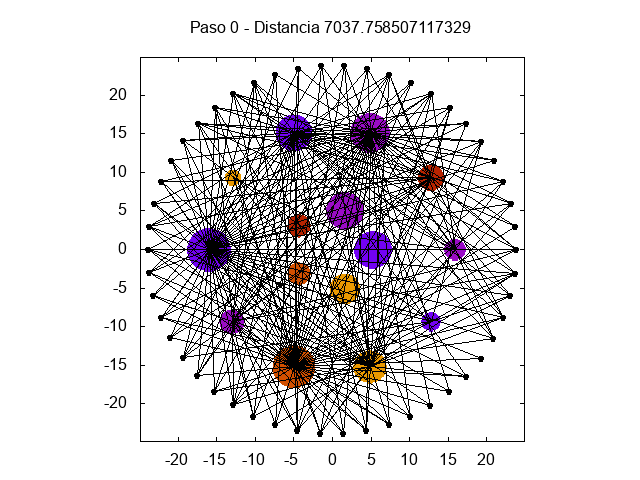
\includegraphics[width=0.7\textwidth]{h000000}
    \centering
    \caption{Representación de alumnos (nodos en negro), materias (nodos que forman la cirfunferencia intermedia) y horarios (nodos que constituyen la circunferencia interior) y sus relaciones mediante arcos.}
    \label{fig:horarios}
  \end{figure}

  Se eligió esta disposición circular debido a que era posible medir la distancia total de los arcos con el fin de minimizar esta distancia en un algoritmo exhaustivo que recorre todos los nodos de un mismo tipo a la vez y los permuta al azar entre sí mismos, almacenando dicho acomodo para la siguiente iteración solo cuando la nueva distancia total de los arcos es menor a la distancia total almacenada en el conjunto anterior. Con esto, e consiguió una reducción de la distancia de $7037.76$ a $6476.35$. Se dejó correr esta mecánica por un 200 mil pasos y se obtuvo una animación del proceso mediante ImageMagick, la cual puede verse en .

  Como trabajo futuro se desea minimizar el número de veces que dos materias que le interesan a un alumno coincidan en el mismo horario y aplicar un algoritmo genético para mejorar el desempeño en el proceso de minimización de distancias.

  \bibliography{biblio}{}
  \bibliographystyle{plain}

\end{document}
